%\documentclass{beamer}
\documentclass[handout]{beamer}
\usepackage[utf8]{inputenc}
\usepackage[T1]{fontenc}
\title{Visual Analytics, Flocking and Design Processes}
\date[ISPN ’80]{Presentation to Visual Analytics Lab. 2014-05-13}
\author[MJC]{Michael Cumming BArch PhD \texttt{mcumming@ocadu.ca}}

\usetheme{MJC}

\setbeamerfont{page number in head/foot}{}
\setbeamertemplate{footline}[frame number]
\setbeamertemplate{caption}[numbered]

%tikz stuff
\usepackage{tikz}
\usepackage{pgf}
\usetikzlibrary{arrows,shapes,automata}
%\usepackage[pgf]{dot2texi}
\usepackage{graphicx}
\usepackage{caption}
\usepackage{subcaption}
\usepackage{float}

%\bibliographystyle{amsalpha}
\usepackage{natbib}
\bibliographystyle{apalike}
% make bibliography entries smaller
\renewcommand\bibfont{\scriptsize}
% If you have more than one page of references, you want to tell beamer
% to put the continuation section label from the second slide onwards
\setbeamertemplate{frametitle continuation}[from second]

% Now get rid of all the colours
\setbeamercolor*{bibliography entry title}{fg=black}
\setbeamercolor*{bibliography entry author}{fg=black}
\setbeamercolor*{bibliography entry location}{fg=black}
\setbeamercolor*{bibliography entry note}{fg=black}
% and kill the abominable icon
\setbeamertemplate{bibliography item}{}

\begin{document}

\begin{frame}
\titlepage
\end{frame}

\begin{frame}{Summary of Talk}
Version 1
\begin{itemize}
\item Visual Analytics often involve Big Data Sets
\item Big Data Sets usually involve Distributed Action
\item Distributed Action usually results in Emergent Patterns
\end{itemize}
\pause

\bigskip
Version 2
\begin{itemize}
\item Greg van Alstyne's talk last week mentioned Herbert Simon
\item Herbert Simon was a great influence on my work
\item Herbert Simon's (and my) work may connect obliquely with Visual Analytics
%\item Distributed Action implies \emph{Patterns of Interaction}
\end{itemize}

\end{frame}

\begin{frame}{Introduction}
My background
	\begin{itemize}
	\item Architectural practice (mostly in Toronto and Europe)
	\item Academia (Computational design / Computer-aided design)
	\item Ambitious City (Support for bottom-up urban design)
	\item MGDS-PET project at DFI / OCADU (wearable devices to support transmedia narratives)
	\end{itemize}
\end{frame}

\begin{frame}{My Research Interests}
Distribution of Design Processes
\begin{itemize}
\item Should design processes be distributed, with less centralization?
\pause
\item If more people worked on complex design problems, would the results improve?
\pause
\item Can the ideas of open source software development be applied to design in general?

\end{itemize}
\end{frame}

\begin{frame}{One Definition of Visual Analytics}
\begin{quote}
Visual analytics combines automated analysis techniques with interactive
visualizations for an effective understanding, reasoning and decision making on
the basis of very large and complex data sets.
\end{quote}
\citep{keim2008visual}
\end{frame}


\begin{frame}
\begin{figure}
  \begin{center}
  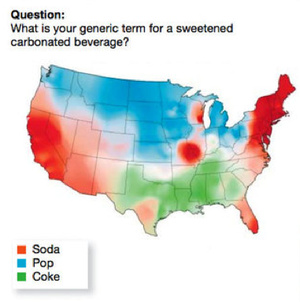
\includegraphics[width=6cm]{images/popSoda.jpg}
  \caption{Carbonated Beverage Linguistic Data}
  %\citep{fung2014how}
  \label{fig:popsoda}
  \end{center}  
\end{figure}
\end{frame}

\begin{frame}{Visual Analytics as an Industrial Technique}
\begin{figure}
\begin{center}
 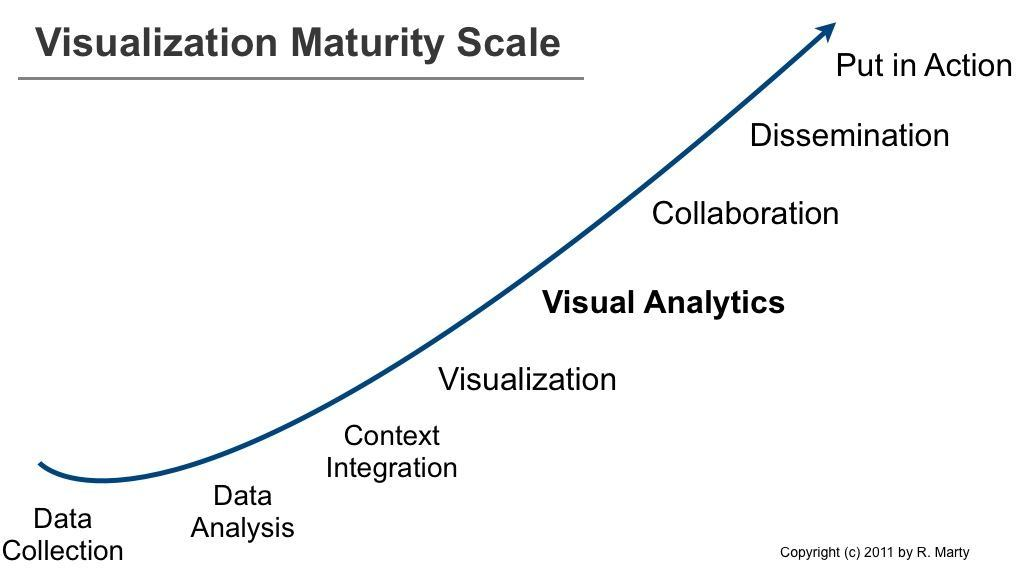
\includegraphics[width=7cm]{images/visMaturity.jpg}
  \caption{Visual Analytics as one step in many data transformations.}
  \label{fig:va}
\end{center}
\end{figure}
\citep{marty2012steps}
\end{frame}

\begin{frame}{Large Data Sets and Distributed Activities}
Large Data Sets are often generated by distributed activities:
	\begin{itemize}
	\item Animals going about their business
	\item People interacting with each other
	\item Particles and waves in nature
	\item Diseases and viruses in a population
	\item Users on the Internet, etc.
	\end{itemize}
\end{frame}

\begin{frame}{Distributed Activities Commonalities}
What do distributed activities have in common?
	\begin{itemize}
	\item Lack of central control
	\item Coordination between independent agents
	\item Independent goal-seeking
	\item Emergent effects
	\end{itemize}
\end{frame}

\begin{frame}{Complexity and Distributed Activities}
\begin{quote}
 When you watch an ant follow a tortuous path across a beach, you might say, "How complicated!" Well, the ant is just trying to go home, and it's got to climb over little sand dunes and around twigs. Its path is generally pointed toward its goal, and its maneuvers are simple, local responses to its environment. To simulate an ant, you don't have to simulate that wiggly path, just the way it responds to obstacles. 
\end{quote}
\citep{simon1994thinking} \citep{simon1996sciences}

\pause
\begin{figure}
\begin{center}
 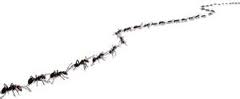
\includegraphics[width=7cm]{images/antTrail02.jpg}
   \caption{}
  \label{fig:antTrail}
\end{center}
\end{figure}

\end{frame}

\begin{frame}{Herbert Simon, 1916-2001}
\begin{figure}
\begin{center}
 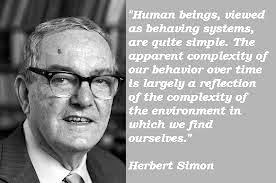
\includegraphics[width=8cm]{images/herbertSimon01.jpg}
    
  \label{fig:herb}
  \citep{simon1996sciences}
  \caption{Pioneering researcher in Artificial Intelligence, Herbert Simon.}
\end{center}
\end{figure}
\end{frame}

\begin{frame}{Ants and People}
\begin{figure}
\begin{center}
 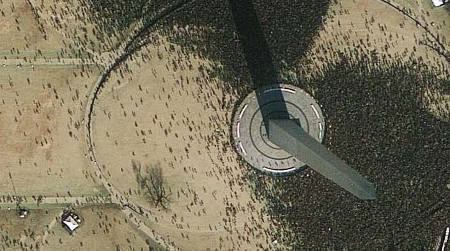
\includegraphics[width=8cm]{images/antsPeople.jpg}
  \caption{Ant-People Descend on Washington, DC.}
  \label{fig:ants}
\end{center}
\end{figure}
\citep{beaton2009ant}
\end{frame}


\begin{frame}{Flocking Birds}
\begin{figure}
  \begin{center}
  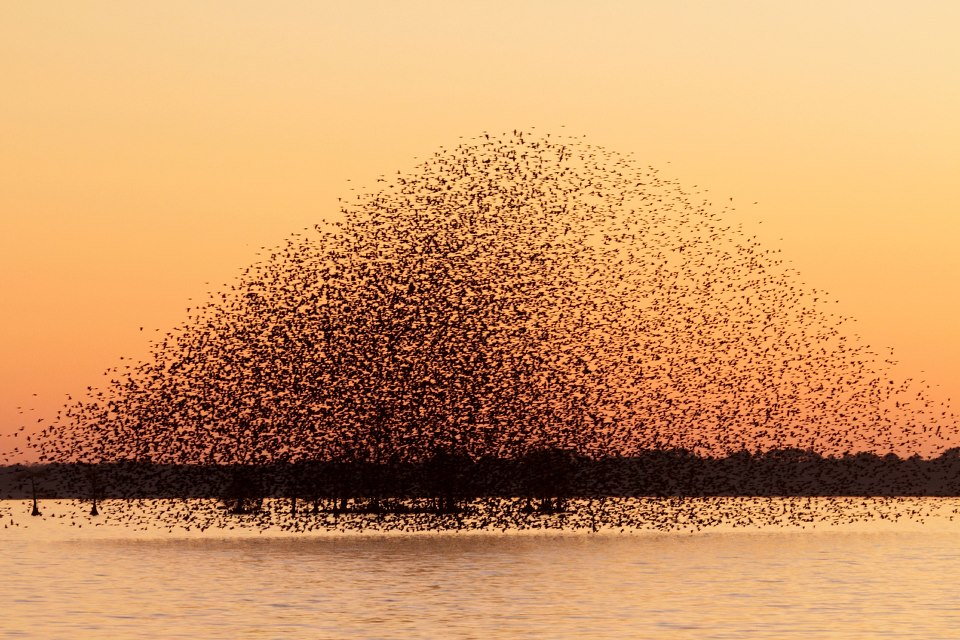
\includegraphics[width=8cm]{images/flocking01.jpg}
  \caption{Flocking red-winged blackbirds over Mattamuskeet Lake in Hyde County, North Carolina (photo by Guy Livesay, 1992)}
  \label{fig:flocking01}
  \end{center}  
\end{figure}
\end{frame}

\begin{frame}{Flocking Rules}
Basic models of flocking behaviour are controlled by three simple rules:
\begin{enumerate}
\item Cohesion: steer towards average position of neighbours (long range attraction)
\item Alignment: steer towards average heading of neighbours
\item Separation: avoid crowding neighbours (short range repulsion)

\end{enumerate}
\citep{reynolds1987flocks}
\end{frame}

\begin{frame}{Flocking Birds: Reynold's Boid Algorithm}
\begin{figure}
  \begin{center}
  \begin{subfigure}[b]{0.3\textwidth}
  
\includegraphics[width=3cm]{images/boid01-cohesion.png}
  \caption{Cohesion}
  \end{subfigure}
    \begin{subfigure}[b]{0.3\textwidth}
    
\includegraphics[width=3cm]{images/boid02-alignment.png}
  \caption{Alignment}
    \end{subfigure}
    \begin{subfigure}[b]{0.3\textwidth}
    
\includegraphics[width=3cm]{images/boid03-separation.png}
  \caption{Separation}
    \end{subfigure}
  \label{fig:boid01}
 \end{center}  
\caption{Boid Rules by Reynolds}
\label{fig:boidRules}  
\end{figure}
\citep{aprk2014boid}
\end{frame}

\begin{frame}{Complex Patterns and Generating Mechanisms}
\begin{block}{Question}Do patterns that look complex or organic always involve simpler, lower-level interactions? [flocking birds / like ants on a beach]
\end{block}
\pause

\begin{block}{Question}Does Visual Analytics study emergent, organic patterns, or the simpler behaviours that may have created them?
\end{block}
\end{frame}
	
\begin{frame}{Collaborative Design as a type of Distributed Activity}
Design is usually done collaboratively.
\bigskip

Why do people collaborate in design?
\begin{itemize}
\item Design problems may be too difficult for single designers
\item Participation required from diverse stakeholders
\item Demands for a range of technical expertise
\item Need for diversity of perspective
\item Requirements for local participation; local knowledge
\end{itemize}
\bigskip
\pause
In order to be able to solve most complex design problems, you need \emph{many minds}.
\end{frame}

\begin{frame}{Coordination Theory, Distributed AI and Collaborative Design}
Three reasons why the actions of multiple agents need to be coordinated: \citep{jennings1996coordination} 
\pause
\begin{enumerate}
\item Because there are dependencies between agents' actions
\pause
\item Because there is a need to meet global constraints, and 
\pause
\item Because no one individual has sufficient competence,
resources, or information to solve the entire problem.
\end{enumerate}
\end{frame}

\begin{frame}{Collaborative design has Centralized and Distributed aspects}
Centralized aspects
\begin{itemize}
	\item Strong design concepts
	\item Team identity; common purpose; common ground
	\item Global attributes of the completed artifact
	\item Total cost
\end{itemize}
\bigskip
\pause
Distributed aspects
\begin{itemize}
	\item Multiple agents, multiple types of expertise, different points of view
	\item Stakeholders` opinions and experiences
	\item Proprietary information
\end{itemize}
\end{frame}



\begin{frame}{Examples: Centralized Design of Cities}
\begin{figure}
\caption{Plan Voisin; Centralized and Distributed City Planning}
 % \begin{center}
  	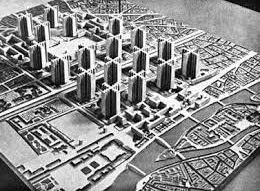
\includegraphics[width=4cm]{images/leCorb01.jpg}
	\pause
    	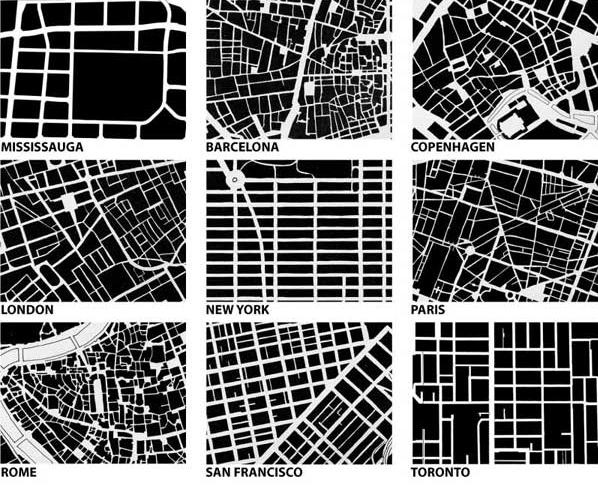
\includegraphics[width=7cm]{images/city-grids.jpg}
      
% \end{center}  
\end{figure}
\end{frame}

\begin{frame}{Examples: Distributed Design of Cities}
\begin{figure}
\caption{Santander, Spain; Toronto Laneway}
%\begin
  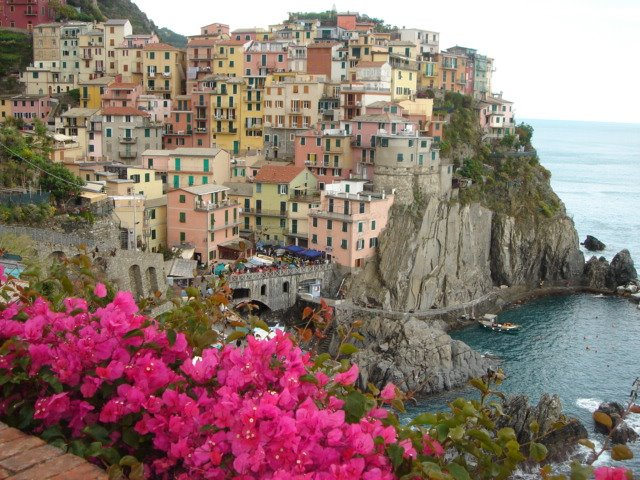
\includegraphics[width=6cm]{images/santander.JPG}
  \pause
    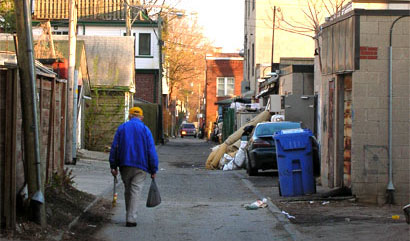
\includegraphics[width=5cm]{images/laneman.jpg}
  
  \label{fig:distributedCity}
 % \end{center}  
\end{figure}
\end{frame}

\begin{frame}{Flocking Rules for Collaborative Designers?}
Boid rules for designers working together in collaborative teams?
\begin{enumerate}
\item Cohesion: steer towards average position of your design collaborators (don`t go too far astray from your collaborators)
\item Alignment: steer towards average heading of your design collaborators (pay attention to where others are going) 
\item Separation: avoid crowding your collaborators (let them do their jobs)
\end{enumerate}
\end{frame}

\begin{frame}{Conclusions}
\begin{itemize}
\item When you have complex, emergent patterns one compact way to understand them is through the algorithms that may have generated them (as with boids). 
\pause
\item Many things that appear to be designed top-down are often unintentional, emergent and dependent on distributed action.
\end{itemize}

\end{frame}

\begin{frame}{References}
\bibliography{mc_references}
\end{frame}

\begin{frame}{Thanks for attending!}
\bigskip
Michael Cumming

\texttt{mcumming@ocadu.ca}

\texttt{michael@ambitiouscity.com}

\end{frame}


\end{document}